\documentclass[conference,a4paper]{IEEEtran}
\IEEEoverridecommandlockouts

\usepackage{cite}
\usepackage{amsmath,amssymb,amsfonts}
\usepackage{algorithmic}
\usepackage{graphicx}
\usepackage{textcomp}
\usepackage{xcolor}
\usepackage{booktabs}

% --- Dual build (ZetaGo_Project_Plan_v2.md SS6) -----------------------------
% \anonfalse -> course build (named authors). \anontrue -> ICCIT CMT build
% (anonymous). Flip this one line, nothing else, before generating either PDF.
\newif\ifanon
\anonfalse

\def\BibTeX{{\rm B\kern-.05em{\sc i\kern-.025em b}\kern-.08em
    T\kern-.1667em\lower.7ex\hbox{E}\kern-.125emX}}

\begin{document}

\title{Do Hand-Engineered Features Still Help? Feature Richness Versus Data
Scale in Supervised 7$\times$7 Go Move Prediction}

\ifanon
\author{\IEEEauthorblockN{Anonymous Authors}
\IEEEauthorblockA{Submission under double-blind review}}
\else
\author{
\IEEEauthorblockN{Mahiul Kabir, Rahatut Tahrim, Obidit Islam}
\IEEEauthorblockA{Department of Computer Science and Engineering \\
Islamic University of Technology \\
Team Sharp Features --- CSE 4622: Machine Learning Lab}
}
\fi

\maketitle

\begin{abstract}
This paper studies whether hand-engineered Go feature planes (stone
liberties, move history) still improve supervised move prediction as
labelled data volume grows, on a controlled 7$\times$7 Go corpus generated
by KataGo self-play. A 3 (feature richness: $N=2,4,7$ planes) $\times$ 4
(data volume) factorial compares classical baselines (logistic regression,
random forest, $k$-NN, linear SVM) against a convolutional policy/value
network. Feature richness and architecture interact rather than combine
additively: the same planes worth $+0.11$ top-1 accuracy to a linear model
are worth $0.0008$ --- below seed noise --- to the CNN, which reaches
$90.4\%$ top-1 / $98.7\%$ top-3 unaided on a sealed test split (mean over 5
seeds, read exactly once) and overtakes every classical baseline once
training data exceeds $\sim$13k unique positions. A
150-game round-robin further shows that PUCT search over the same frozen
weights adds strength ($\approx$400 Elo, $p{=}4.1{\times}10^{-3}$)
substantially exceeding any single supervised-learning design choice in
the study. All data, code, and analysis scripts are
publicly available\ifanon{} (link withheld for review)\else{} at
\texttt{[repository URL withheld pending release]}\fi.
\end{abstract}

\begin{IEEEkeywords}
Go, supervised learning, feature engineering, data scarcity, convolutional
neural networks, ablation study
\end{IEEEkeywords}

\section{Introduction}
\label{sec:intro}
As labelled self-play data grows, does hand-engineered structure
(liberties, move history) still earn its keep against a model that can in
principle learn the same structure from raw stone positions given enough
data? This paper's contributions are:
\begin{enumerate}
  \item A controlled 3$\times$4 factorial ablation isolating feature
    richness from data volume on a single, oracle-verified 7$\times$7 Go
    corpus (120{,}000 KataGo self-play games).
  \item A comparison of four classical baselines and a CNN policy/value
    network, compute-matched, with a properly-derived baseline for every
    metric (majority-class/uniform-random for policy, side-to-move for
    value) --- a step several move-prediction papers skip.
  \item An honest accounting of a small-board corpus's information ceiling:
    56{,}798 unique positions out of 3.3M rows, and what that means for a
    data-volume factor.
  \item A compute-cheap unsupervised sub-study (\S\ref{sec:track_b}): an
    autoencoder, classical clustering, and control-paired linear probes ask
    whether reconstruction alone recovers the same board structure
    supervision does.
\end{enumerate}
Related work is reviewed in \S\ref{sec:related}, the corpus and experimental
design in \S\ref{sec:dataset}--\ref{sec:methodology}, results in
\S\ref{sec:results}, and their implications in \S\ref{sec:discussion}.

\section{Related Work}
\label{sec:related}
\textit{Search-guided self-play for Go and chess.} AlphaGo
\cite{silver2016mastering} combined supervised policy pretraining with
MCTS and RL; AlphaGo Zero \cite{silver2017mastering} and AlphaZero
\cite{silver2018general} removed human data entirely. KataGo
\cite{wu2019accelerating} is the methodological ancestor of this paper's
data pipeline and the source of its labels (\S\ref{sec:dataset}); its
ablations on auxiliary targets and input features are the closest precedent
for a controlled feature-richness study, at much larger scale and board
size. Kocsis and Szepesv\'ari's UCT \cite{kocsis2006bandit} underlies the
tree search above, and MCTS feature-biasing work \cite{soemers2019biasing}
is the closest general-game-playing analogue of Factor A: linear feature
weights instead of a full network.

\textit{Supervised pattern learning without search.} DeepChess
\cite{david2016deepchess} is the nearest analogue for this paper's
supervised-only framing: an end-to-end network trained purely on positions
and outcomes. Interpretability work on search-free and search-trained game
engines --- concept probing in AlphaZero \cite{mcgrath2022acquisition},
representation quality in chess vision transformers
\cite{czech2023representation}, and the control-task methodology for
validating that a probe measures signal rather than capacity
\cite{hewitt2019designing} --- motivates this paper's insistence on
properly-derived baselines (\S\ref{sec:methodology}): a probe or classifier
beating a carelessly-chosen baseline is the same failure mode in either
literature.

\textit{Small-board Go and classical feature selection.} Small-board Go has
an established solved-game literature \cite{vanderwerf2003solving},
grounding $7{\times}7$ as tractable for full self-play yet still
combinatorially non-trivial. Feature richness sits in classical
feature-selection theory \cite{guyon2003introduction} and pattern-recognition
grounding \cite{bishop2006pattern}: features help only when a model cannot
already infer their content from raw input, exactly Factor B's question.

\section{Dataset}
\label{sec:dataset}

\subsection{Generation}
The corpus is 120{,}000 self-play games generated by KataGo v1.16.5
(Eigen/CPU build) via its \texttt{match} subcommand, at \texttt{maxVisits =
16}, single search thread, network
\texttt{g170e-b10c128-s1141046784-d204142634}. Rules are fixed and identical
in generation and replay: board $7\times7$, komi $9.5$, positional superko,
area (Tromp--Taylor) scoring, multi-stone suicide illegal; zero games were
dropped for a rule or board-size mismatch.

\subsection{Splits}
All three splits (Table~\ref{tab:splits}) are carved from this single
120{,}000-game run and partitioned \emph{by game} (never by position) via
$\mathrm{crc32}(\texttt{file:line}) \bmod 20$, which is what guarantees zero
game overlap between splits --- splitting by position would leak, since
positions within a game are highly correlated.

\begin{table}[t]
\centering
\caption{Train/val/test split. All three carved from one generation run;
game-level overlap verified $=0$ for every pair.}
\label{tab:splits}
\begin{tabular}{lrrr}
\toprule
Split & Games & Positions & Share \\
\midrule
Train & 107{,}969 & 3{,}310{,}156 & 90.0\% \\
Val & 6{,}027 & 184{,}834 & 5.0\% \\
Test (sealed) & 6{,}004 & 182{,}102 & 5.0\% \\
\bottomrule
\end{tabular}
\end{table}

The test split is touched exactly once, for the final results table; every
tuning and model-selection decision in this paper uses the validation
split.

\subsection{Policy label}
The task is 50-way classification (49 board points + pass). Contrary to an
earlier design assumption favouring centre/tengen dominance, the board-point
distribution is comparatively flat: the most frequent point (centre,
$3.29\%$) is only $4.4\times$ the least frequent ($0.75\%$). The one
genuinely outsized class is \texttt{pass} itself, the training-set mode at
$9.09\%$ (Fig.~\ref{fig:classdist}). Macro-F1 is reported throughout on this
basis --- ``50-way classification whose largest class is pass,'' not severe
imbalance.

\subsection{Value label: a baseline trap}
\label{sec:valuetrap}
White wins $90.6\%$ of games at the game level --- not a defect: removing
komi from final scores shows $71\%$ of games settle at exactly margin $+9$,
the established solved value of $7\times7$ Go under perfect play. Komi
$9.5$ (half a point above $9$, so no game draws) then hands those games to
White by the minimum margin. This is a spike in the outcome distribution,
not a spread, so no komi value rebalances it without changing which side
wins by construction; $9.5$ is kept and the skew is reported, not engineered
away.

The consequence for evaluation is a value-label baseline trap. Since
\texttt{values} is stored from the side-to-move's perspective and side
alternates every ply, row-level balance looks fair (train: $49.4\%$ win /
$50.6\%$ loss) while a much stronger regularity holds at the level that
matters: predicting a win iff White is to move scores $85.84\%$ (train) /
$85.55\%$ (val) / $86.44\%$ (test) accuracy alone. Scoring against the
$50.6\%$ marginal-majority baseline instead would overstate any result by
roughly 35 points. Every value accuracy here is quoted beside the $85.55\%$
validation-split side-to-move
baseline for this reason (see also \S\ref{sec:methodology} for the
consequence this has for the value \emph{target}, not just the baseline).

\subsection{Duplication and train/val position overlap}
\label{sec:duplication}
Two properties of the corpus would otherwise surface as reviewer objections
and are disclosed here directly. First, the corpus is small in
\emph{unique} positions relative to its row count: the full training split
holds $3{,}310{,}156$ rows but only $56{,}798$ unique board states, a
$58.3\times$ duplication factor, concentrated almost entirely in the opening
and not a corpus-wide defect: plies 0--6 supply $22.8\%$ of all rows but only
$93$ of $56{,}798$ unique positions ($0.2\%$, each repeated roughly $8{,}100$
times), while plies 20 and beyond supply $91.7\%$ of unique positions at
roughly $22\times$ repetition --- in unique-position terms the corpus is
$92\%$ midgame and endgame content. Training on raw rows would let the $93$
opening boards dominate roughly a quarter of every gradient step, diluting
any measured feature-richness effect (liberty and history planes carry almost
no information on a near-empty board); \S\ref{sec:methodology}'s featurisation
is therefore always evaluated at natural, non-deduplicated row weighting, an
asymmetry the reader should weigh at the smallest data-volume levels.

Second, $90.7\%$ of validation rows hold a board position that also occurs
in train. This is \emph{not} leakage --- game-level overlap is exactly zero,
verified directly --- but the ordinary structure of a shared opening book:
every game begins from the same first move (only 17 distinct positions by
ply 4), so overlap starts at $100\%$ for ply $<10$ and decays monotonically
as the tree branches, to $90.2\%$ by ply 20--30 and $50.4\%$ by ply 50+.
Opening-move determinism (not addressed here; the tested-safe remedy is
randomising the first plies before self-play) is the underlying cause of
both this and the row-weighting skew above.

\begin{figure}[t]
  \centering
  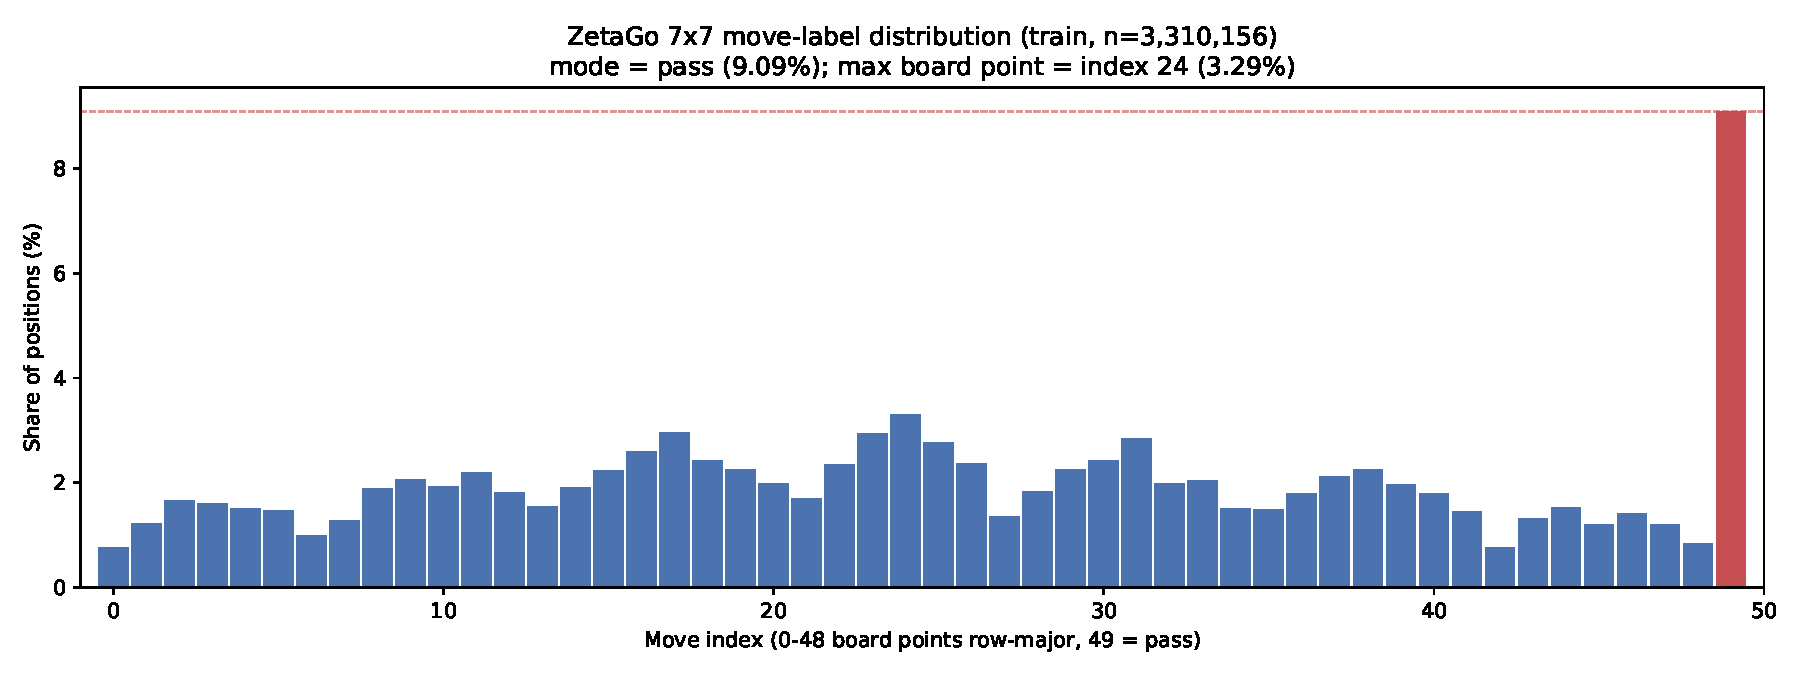
\includegraphics[width=0.82\linewidth]{figures/class_distribution.pdf}
  \caption{Move-label distribution, training split ($n=3{,}310{,}156$). Mode
  is \texttt{pass} (9.09\%), not a board point; board-point distribution is
  comparatively flat (max 3.29\%, centre). Basis for macro-F1 as ``50-way
  classification whose largest class is pass,'' not severe imbalance.}
  \label{fig:classdist}
\end{figure}

\section{Methodology}
\label{sec:methodology}
We formally define the two experimental factors, the model set, the
prediction targets, and the evaluation protocol below.
\begin{itemize}
  \item \textbf{Factor A (feature richness).} $N=2$: current-player and
    opponent stone planes. $N=4$: $N=2$ + normalised group liberties +
    turn indicator. $N=7$: $N=4$ + signed history at $t-1$/$t-2$ (both
    players' stones, not just the mover's own) + an occupancy-change plane.
  \item \textbf{Factor B (data volume).} Nested by-game nested subsamples:
    1{,}000 / 5{,}000 / 20{,}000 / 107{,}969 (full) games, corresponding to
    5{,}501 / 12{,}748 / 24{,}277 / 56{,}798 unique positions --- state both
    quantities; reporting rows alone misrepresents information content by
    $\sim$58$\times$.
  \item \textbf{Models.} Logistic regression, random forest, $k$-NN, and
    linear SVM (flattened, all four compute-matched at 80k rows), plus a
    three-layer convolutional policy/value network on the full split.
  \item \textbf{Value target.} Score margin (regression), not win/loss:
    \S\ref{sec:valuetrap} shows win/loss is near-solved (side-to-move
    baseline $85.84\%$ train / $85.55\%$ val) while the same rule explains
    only $8.1\%$ of margin variance, so margin is the non-degenerate target
    our value head regresses --- the same quantity KataGo's own value head
    predicts. MSE floors any margin model must clear: $265.73$ (predict $0$),
    $244.09$ (best constant per side-to-move). Win/loss is still reported as
    the derived sign of the predicted margin, beside the $85.55\%$ baseline.
  \item \textbf{Baselines.} Majority-class and uniform-random-over-legal for
    policy; side-to-move ($85.55\%$ val) for value, not the marginal-majority
    baseline ($50.6\%$), which would overstate any result by $\sim$35 points.
  \item \textbf{Seeds and CIs.} 5 seeds per cell; 95\% bootstrap confidence
    intervals resampled over \emph{games}, not positions, since positions
    within a game are correlated.
\end{itemize}

\subsection{Search-augmented evaluation}
\label{sec:mctsmethod}
Beyond the supervised factorial, we evaluate whether search over a frozen,
already-trained model improves playing strength relative to a one-shot
policy read. We use PUCT \cite{kocsis2006bandit,silver2016mastering},
selecting by $Q + c_{\mathrm{puct}} \cdot P \cdot \sqrt{N_{\mathrm{parent}}} /
(1+N_{\mathrm{child}})$ down to an unexpanded leaf, evaluated once by the
frozen network (policy head as prior, masked to legal moves and renormalised;
value head's margin as leaf value, negated when propagated to the opponent's
node); terminal nodes use the true Tromp--Taylor outcome. The root's move is
the highest visit count after $N{=}100$ simulations at $c_{\mathrm{puct}}{=}1.5$
(configuration, not tuned). The greedy baseline's pass rule (a move-history
minimum before pass is eligible, since \texttt{pass} is the modal training
label) applies at every search node, evaluated at that node's own ply.

Search here is strictly \emph{evaluation-time}: no weight update, gradient
step, or reward signal occurs, and no simulated game is ever recorded as
training data --- the design boundary separating this from AlphaZero-style
self-play, which would retrain on search-generated targets. No Dirichlet
root noise is applied, since that is a training-time exploration device with
no role in a pure strongest-move search.

Three agent tiers share one trained model: uniform-random over legal moves;
one-shot greedy (argmax, same pass rule); and the PUCT agent above. Greedy
and search wrap \emph{identical} weights, so any gap between them is
attributable to search alone (Section~\ref{sec:results}). Agents meet in a
round-robin with equal games per colour per pair --- mandatory, since
\S\ref{sec:valuetrap} shows colour explains more of a game's outcome here
than either agent's skill. Strength is a Bradley--Terry Elo rating with
bootstrap CIs, anchored at random, alongside head-to-head records: an anchor
swept without a loss drives its own strength to zero and every Elo to
$+\infty$, so head-to-head is reported alongside Elo, not instead of it.

Both greedy and search are deterministic given a fixed model, so repeated
games between the same pair are not independent trials unless the opening
varies. We prepend a small number of uniformly random legal moves before
either agent takes control, drawn independently per repetition and shared
between both colour assignments of that repetition, preserving colour
balance position-for-position.

\subsection{Unsupervised representation}
\label{sec:track_b_method}
Separately, we ask whether a convolutional autoencoder trained on raw stone
positions alone recovers board structure comparable to the supervised CNN's,
and whether its weights transfer \cite{hinton2006reducing}. The encoder is
the champion CNN's body verbatim (three $3{\times}3$ same-padded
convolutions, $64$ channels, so weights are transplantable,
\S\ref{sec:track_b}), projected to a latent of $64$ (dimension-matched to the
value head's own penultimate layer) or, secondarily, $32$; the decoder
mirrors this in reverse, trained with BCE-with-logits on the raw $N{=}2$
stone-occupancy planes. It never receives \texttt{moves}, \texttt{values}, or
\texttt{margins} (a runtime assertion, not convention) and always trains
deduplicated (\S\ref{sec:dedupablation}'s \texttt{dedup=unique}, here
mandatory: $56{,}798$ unique positions, $10\%$ held out for reconstruction-loss
model selection only). For each board statistic (stone count, move number,
largest/atari group counts, mean distance from centre) we fit a linear probe
from a $64$-d latent to that statistic, paired with a control trained
identically against a row-shuffled target \cite{hewitt2019designing}: a probe
that does not clear its control demonstrates probe capacity, not structure.
$k$-means (silhouette-selected $k$) and DBSCAN on a PCA-reduced space
($90\%$-variance components; $\varepsilon$ from a fixed nearest-neighbour
heuristic, never tuned post hoc) cluster encoded validation positions, with
stability checked by adjusted Rand index across 3 autoencoder seeds. The
identical protocol then runs, unchanged, on the champion CNN's own $64$-d
value-head penultimate layer.

\section{Results}
\label{sec:results}

\subsection{Move prediction}
The headline number is on the sealed test split, read exactly once, after
every design and model-selection decision below was frozen on validation.
The full-volume N=4 cell was retrained at 5 seeds for this pass (distinct
from \S\ref{sec:mctsresults}/\S\ref{sec:track_b}'s persisted champion ---
GPU/CPU nondeterminism, \S\ref{sec:discussion}); its seed-46 instance scores
$90.46\%$/$98.72\%$/$91.70\%$ (top-1/top-3/macro-F1) on test against
$90.40\%$/$98.72\%$/$91.60\%$ on validation, the same weights --- no
generalisation gap. Table~\ref{tab:testresults} gives all five models on
test; every other result (Table~\ref{tab:top1} onward) is validation, since
Factor A/B and the tournament were run once, on validation, by design.

\begin{table}[t]
\centering
\caption{Test-set results, full volume, N=4, 5 seeds (mean$\pm$SD), read
exactly once after all decisions were frozen on validation.}
\label{tab:testresults}
\begin{tabular}{lrrr}
\toprule
Model & Top-1 & Top-3 & Macro-F1 \\
\midrule
logreg & $0.7963\pm0.0017$ & 0.9196 & 0.7952 \\
rf & $0.8752\pm0.0003$ & 0.9600 & 0.8826 \\
knn & $0.8137\pm0.0030$ & 0.9364 & 0.8110 \\
svm & $0.7912\pm0.0014$ & 0.9157 & 0.7878 \\
cnn & $\mathbf{0.9037\pm0.0005}$ & \textbf{0.9872} & \textbf{0.9158} \\
\bottomrule
\end{tabular}
\end{table}

An exact McNemar test (CNN vs.\ RF, seed 46) confirms the crossover below on
identical positions: of $8{,}847$ test disagreements, CNN is right and RF
wrong on $7{,}130$, the reverse on $1{,}717$ ($p<10^{-300}$); the same
asymmetry holds on validation ($6{,}986$ vs.\ $1{,}839$ of $8{,}825$,
$p<10^{-300}$) --- not a validation-set artefact. Table~\ref{tab:top1}
reports mean top-1 across seeds/encodings for every (model, volume) cell on
validation.

\begin{table}[t]
\centering
\caption{Mean top-1 accuracy by model and data volume (5 seeds, 3
encodings). Bold marks the row maximum.}
\label{tab:top1}
\begin{tabular}{lrrrr}
\toprule
Model & 1k & 5k & 20k & full (108k) \\
\midrule
logreg & 0.7711 & 0.7899 & 0.7899 & 0.7901 \\
rf & 0.8589 & \textbf{0.8775} & 0.8759 & 0.8760 \\
knn & 0.7676 & 0.8123 & 0.8120 & 0.8143 \\
svm & 0.7726 & 0.7798 & 0.7802 & 0.7795 \\
cnn & 0.8192 & 0.8764 & 0.8934 & \textbf{0.9036} \\
\bottomrule
\end{tabular}
\end{table}

Every classical model captures essentially its full gain between 1k and 5k
games and is flat thereafter; the CNN keeps improving to the last data
point. Fig.~\ref{fig:learning} plots the same result against \emph{unique}
training positions rather than games sampled --- the axis that actually
varies information content, since $108\times$ more games buys only
$10.9\times$ more unique positions (\S\ref{sec:duplication}). Random forest leads below $\sim$13k unique positions; the CNN overtakes it
once unique coverage passes that point and the gap widens monotonically.
Checked per seed rather than on pooled means, all five agree on the ranking
at 20k and full volume (wide, consistent CNN margin); at 5k RF leads on
$4/5$ seeds but by at most $0.004$ --- an order of magnitude below its
unambiguous $0.040$ lead at 1k --- so we read 5k as the crossover's
near-boundary, with the CNN advantage dominating only from 20k onward.

\begin{figure}[t]
  \centering
  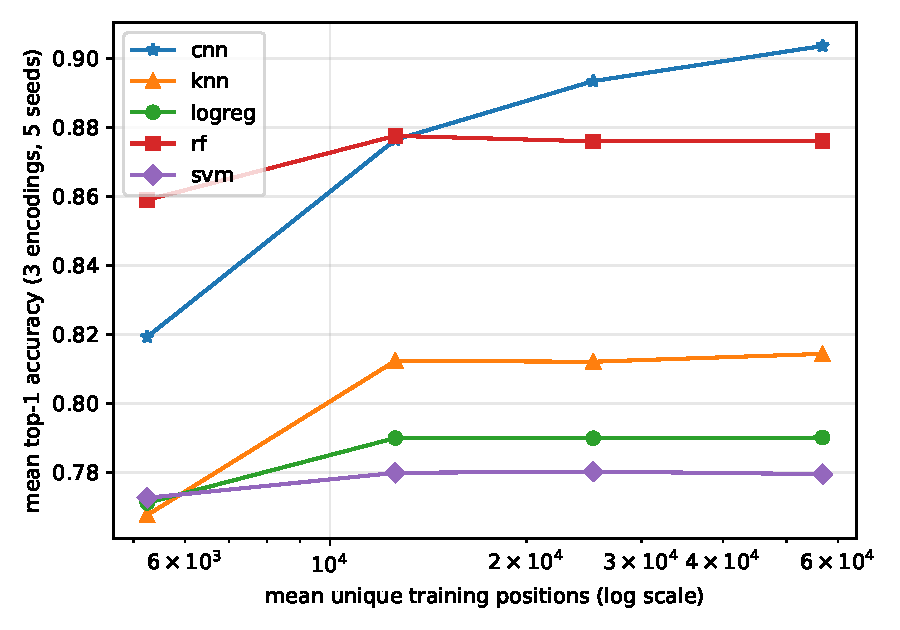
\includegraphics[width=0.82\linewidth]{figures/learning_curve.pdf}
  \caption{Mean top-1 accuracy vs.\ mean unique training positions (log
  scale), one line per model, mean over 3 encodings and 5 seeds. Classical
  models plateau by $\sim$13k unique positions; the CNN does not.}
  \label{fig:learning}
\end{figure}

\subsection{Feature richness (Factor A)}
\label{sec:factorA}
Comparing each model's $N{=}2{\to}N{=}7$ spread in top-1 at full volume
against its own across-seed standard deviation isolates whether feature
richness helps at all, and for which models. SVM moves by $0.1095$
($70\times$ its seed SD of $0.00156$); logistic regression by $0.0900$
($77\times$ its SD of $0.00117$). Random forest moves by only $0.0021$
(above noise but small); $k$-NN's $0.0032$ spread sits inside its own SD.
The CNN's spread is $0.0008$ --- \emph{below} its seed SD of $0.00081$, and
below a quarter of the mean bootstrap confidence-interval width on any
single one of these rows ($0.0032$). The identical featuriser, data, and
protocol that moved SVM by $145\times$ the CNN's spread confirms this null
is a property of the model, not an underpowered experiment: liberty counts
and history planes are worth roughly $+0.10$ top-1 to a linear model and
nothing measurable to the convolutional network, which apparently recovers
the same information from raw stone positions through its own early
layers. A two-way ANOVA on top-1 (factors: encoding, model; full volume, 5
seeds) confirms this formally: the encoding$\times$model interaction term is
significant at $F(8,60){=}1295$, $p<10^{-60}$ --- feature richness's effect
genuinely depends on which model receives it, not an artefact of comparing
effect sizes to noise floors informally.

\subsection{Value target}
The CNN has the lowest margin MSE ($69.78$ vs.\ RF's $72.31$, full volume)
but RF has the higher win/loss sign accuracy ($93.17\%$ vs.\ $91.71\%$,
baseline $85.55\%$) --- the same pattern replicates on test
(\S\ref{sec:results}: RF $0.9343$ vs.\ CNN $0.9206$). Different quantities:
the CNN fits its regression target more precisely overall, RF is more often
correct about which side of zero the margin falls on; a model can lead on
one and trail the other, so both are reported.

\subsection{Error analysis}
A literal $50{\times}50$ confusion matrix is unreadable and almost entirely
zeros; Fig.~\ref{fig:recall} instead plots its diagonal --- per-true-point
top-1 recall --- on board geometry, more informative for a spatial task. The
centre (index 24) recalls at $99.9\%$; its four orthogonal neighbours are the
worst points on the board (as low as $59.0\%$), and the dominant confusions
are between centre and these neighbours (the single most common error,
$0.78\%$ of rows, is true $=$(row 3, col 2) predicted (row 2, col 3), both
one step from centre). \texttt{pass} (50th class) recalls at $93.0\%$
($n{=}16{,}849$). Consistent with the $8.3$-point top-1/top-3 gap: most
residual error is not confusing strong moves with weak, but ranking among
several similarly strong central points, several simultaneously reasonable
in $7\times7$ play.

\begin{figure}[t]
  \centering
  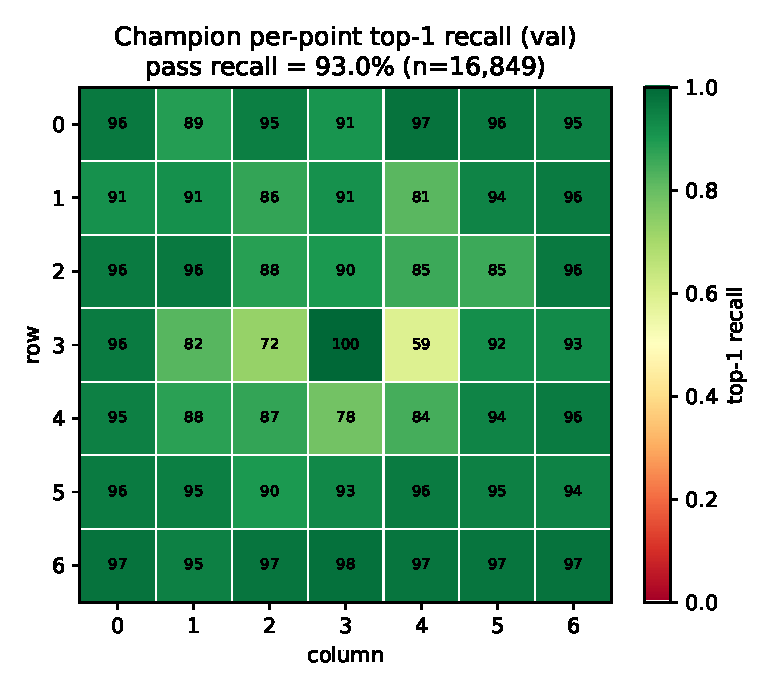
\includegraphics[width=0.85\linewidth]{figures/recall_heatmap.pdf}
  \caption{Per-point top-1 recall, champion model (val) --- diagonal of the
  50-class confusion matrix on board geometry. \texttt{pass} (93.0\% recall,
  $n{=}16{,}849$) is the 50th class, not shown. Error concentrates on the
  centre's immediate neighbours, not distant points.}
  \label{fig:recall}
\end{figure}

\subsection{Search-augmented playing strength}
\label{sec:mctsresults}
The greedy and search agents (\S\ref{sec:mctsmethod}) wrap the identical
champion weights, so any strength gap is attributable to search alone.
Table~\ref{tab:tournament} reports the 150-game round-robin.

\begin{table}[t]
\centering
\caption{Round-robin strength, 25 games/colour/pair, 4 random opening
plies. Elo anchored at \texttt{random}.}
\label{tab:tournament}
\begin{tabular}{lrrr}
\toprule
Agent & Win rate & Elo & 95\% CI \\
\midrule
mcts (100 sim) & 0.950 & 802.8 & [633.0, 1161.2] \\
greedy (argmax) & 0.500 & 401.4 & [268.5, 588.3] \\
random & 0.050 & 0.0 & --- \\
\bottomrule
\end{tabular}
\end{table}

Head-to-head: mcts defeats greedy $45$--$5$, Elo CIs non-overlapping. The 50
games per pair are 25 openings played both colours, so scored per opening:
mcts sweeps 20 of 25, splits 5, greedy sweeps \emph{zero}. An exact binomial
on sweeps alone (most conservative, discarding the 5 splits) gives
$p{=}4.1\times10^{-3}$. The $\approx$400-Elo gap between search and one-shot
argmax on identical weights exceeds every supervised-learning effect above.

A first version without opening randomisation reported mcts 50--0: since
both agents are deterministic (argmax; no exploration noise), those 50 games
were 2 distinct games replayed 25 times each. Discarded, reported here only
with randomised openings --- a pitfall worth flagging for any deterministic
game-playing evaluation, not specific to this corpus.

\subsection{Duplication ablation}
\label{sec:dedupablation}
\S\ref{sec:duplication} leaves open whether the CNN's data-volume gain is
genuinely more information or just more exposure to repeated opening rows.
Retraining the champion cell with \texttt{dedup=unique} ($56{,}798$ rows for
$3{,}310{,}156$) at the same 12 epochs costs $0.223$ top-1
($0.9040\to0.6812$) --- large enough that Table~\ref{tab:top1}'s Factor B
result could be an artefact of opening rows dominating gradient steps.
Extending to $100$ epochs ($58\times$ fewer steps/epoch) closes $89\%$ of
that gap (residual $0.024$) --- not catch-up, since its training loss
($0.204$) is already \emph{lower} than the 12-epoch raw model's ($0.383$)
while validation top-1 stays below it: overfitting a uniform training
distribution evaluated against a frequency-weighted one. We read Factor B as
dominated by gradient-step budget, with a smaller residual gap from
train/val distribution matching, not duplication itself.

\subsection{Unsupervised representation}
\label{sec:track_b}
At latent $64$ the autoencoder reaches near-lossless reconstruction (holdout
BCE $1.0{\times}10^{-7}$, train/holdout tracking together); at $32$ it
plateaus five orders of magnitude higher ($0.0139$) --- a real bottleneck.
Table~\ref{tab:probes} shows the two families diverging sharply on linear
probes (control $R^2 \in [-0.02, 0.00]$ throughout, omitted for space; every
probe clears it): the autoencoder recovers simple global statistics almost
perfectly, the supervised representation far more weakly --- reconstruction
cannot discard occupancy detail without cost; a value head can discard
whatever does not help predict the outcome, and does.

\begin{table}[t]
\centering
\caption{Linear-probe $R^2$ recovering board statistics from a $64$-d latent.
Every control $R^2$ (shuffled target, identical protocol) is in $[-0.02,
0.00]$; every probe below clears it.}
\label{tab:probes}
\begin{tabular}{lrrr}
\toprule
Statistic & AE ($L{=}64$) & AE ($L{=}32$) & Champion (N=4) \\
\midrule
Stone count & 0.979 & 0.943 & 0.268 \\
Move number & 0.825 & 0.801 & 0.501 \\
Largest group & 0.479 & 0.480 & 0.155 \\
Group count & 0.161 & 0.052 & 0.108 \\
Groups in atari & 0.087 & 0.036 & 0.062 \\
Edge-vs-centre & 0.849 & 0.814 & 0.271 \\
\bottomrule
\end{tabular}
\end{table}

Cluster geometry inverts this: the champion has a clean silhouette optimum at
$k{=}3$ ($0.468$; one $93.0\%$ cluster plus two small late-game clusters,
mean move number $\approx$54 vs.\ $30.6$ overall), while no autoencoder run
($2$ latents $\times$ 3 seeds) ever finds an interior peak --- silhouette
still rises at $k{=}20$, our ceiling, at a best value ($0.16$) a third of the
champion's. Assignment is nonetheless fairly stable across seeds (adjusted
Rand $0.73$--$0.83$): reproducible, just not well-separated. DBSCAN agrees
($16$ clusters/$38\%$ noise for the champion vs.\ $101$--$120$ fragments per
autoencoder run) on a PCA space needing more components for $90\%$ variance
($32$--$33$ of $64$ vs.\ the champion's $22$) --- supervision compresses to
lower effective dimensionality here.

Copying the latent-$64$ encoder's three conv layers into a fresh N=2 CNN,
trained at the smallest volume ($1{,}000$ games, $5$ seeds, both arms local
to avoid \S\ref{sec:discussion}'s GPU/CPU drift) gives a positive but
inconclusive edge over random init ($0.8280\pm0.0058 \to 0.8334\pm0.0035$
top-1, $t(4){=}1.55$, $p{=}0.20$; $0.7554\pm0.0370 \to 0.8076\pm0.0576$ value
accuracy, $t(4){=}2.03$, $p{=}0.11$) --- one row, not a second headline.

\section{Discussion}
\label{sec:discussion}

\textbf{The CNN-vs-classical comparison is confounded by architecture, not
just capacity.} A linear model over flattened pixels cannot represent a
translation-equivariant filter regardless of data, so Table~\ref{tab:top1}
and Fig.~\ref{fig:learning} should be read as \emph{feature richness vs.\
architecture-appropriate capacity}, not convolution being unconditionally
superior: \S\ref{sec:factorA} shows the same planes are worth a large, real
amount to linear models precisely because they lack the inductive bias to
derive that structure themselves.

\textbf{The crossover's dynamic range is bounded by the corpus.} $108\times$
more games buys only $10.9\times$ more unique positions
(\S\ref{sec:duplication}), so Factor B spans roughly one order of magnitude
in the quantity that matters; the CNN was still gaining at the last data
point (Table~\ref{tab:top1}), so the reported crossover is a lower bound,
not an observed plateau.

\textbf{Reproducibility has two distinct failure modes, not one.} The corpus
is not bit-reproducible on regeneration (KataGo seeds per run), so exact
replication needs our released HDF5 files, not just our generation config.
Separately, GPU training is not bit-reproducible from identical seeds and
code: the released checkpoint measures $90.40\%$ top-1 against $90.46\%$ for
the sweep cell it was re-trained from (same seed, same hyperparameters). Any
number here should be read with a $\pm0.06$-point band from this source
alone, on top of our confidence intervals' seed-to-seed spread.

\textbf{The teacher bounds both what ``move prediction'' can mean and how
noisy our playing-strength instrument is.} Every label comes from one
KataGo network at \texttt{maxVisits=16}; a $90\%$ top-1 model imitates that
policy well, not optimal $7\times7$ play, and a stronger teacher would raise
every model's ceiling here. Separately, \S\ref{sec:valuetrap} shows $71\%$
of self-play games share one outcome; colour-balanced round-robin
(\S\ref{sec:mctsmethod}) mitigates this, but head-to-head play between two
\emph{weak} agents still varies more than KataGo's own strong self-play ---
our search agent lost 5 of 50 games to one-shot argmax despite a
$\approx$400-Elo gap, a noisy instrument, not a broken one.

\textbf{Reconstruction and supervision preserve different information, not a
strictly better or worse representation.} \S\ref{sec:track_b}'s autoencoder
recovers raw board statistics the same-dimensional supervised representation
does not, while that representation clusters far more cleanly. With
\S\ref{sec:factorA}'s finding that the CNN needs no hand-engineered liberty
or history planes, both results describe the same architecture from opposite
directions: given a target, it discards detail that target does not need;
given none, it keeps everything it can.

\textbf{Two properties of the corpus are disclosed rather than fixed}
(\S\ref{sec:duplication}): opening-move determinism (only 17 distinct
positions exist by ply 4) and the resulting $90.7\%$ train/val position
overlap. Neither is leakage --- game-level overlap is exactly zero --- but
both compress diversity in the low-ply region, which is also where Factor
A's planes carry the least information; some of the small-volume regime's
flatness for classical models may owe to this, not capacity alone.

\section{Conclusion}
\label{sec:conclusion}
This paper set out to ask whether hand-engineered Go feature planes still earn
their keep as labelled data grows, on a controlled, oracle-verified
$7\times7$ corpus. The answer is architecture-dependent rather than uniform:
liberty and history planes buy a linear model up to $+0.11$ top-1 accuracy
and buy a three-layer CNN nothing measurable, an interaction confirmed by a
two-way ANOVA on encoding $\times$ model ($p<10^{-60}$ on the interaction
term), not just an effect-size argument. The same CNN reaches $90.4\%$ top-1
move prediction unaided on the sealed test split, overtakes every classical
baseline once training data exceeds $\sim$13k unique positions, and gains
substantially more from
search over its own frozen weights ($\approx$400 Elo) than from any
supervised-learning design choice in the study. A compute-cheap unsupervised
sub-study asked a parallel question of the same architecture: a
reconstruction-trained autoencoder recovers raw board statistics a
same-dimensional supervised representation does not, while that supervised
representation organises into far cleaner clusters --- reconstruction and
supervision preserve different information about the same board, not one
subsuming the other.

Three stated limitations bound how far this generalises: every label comes
from one fixed KataGo teacher, so the study measures imitation of one
policy, not optimal play; opening-move determinism compresses diversity
exactly where Factor A's planes carry least information; and the AE-init
transfer result (\S\ref{sec:track_b}) is directionally positive but
underpowered at five seeds. Future work, in priority order: a
higher-\texttt{maxVisits} teacher to raise every model's ceiling here;
randomised opening plies during generation, decoupling genuine diversity
from the opening-book artifact; and a larger-$n$ transfer-ablation re-run,
deliberately scoped here as one row, not a second headline.

\section*{Acknowledgment}
\ifanon
  Withheld for double-blind review.
\else
  The authors thank the course instructor for guidance and Kaggle for
  training compute.
\fi

\section*{AI Usage Statement}
Generative AI (Claude, Anthropic) was used for code debugging, concept
explanation, and proofreading, per Guidelines v1.1's permitted uses; it did
not write the manuscript prose. All analysis, interpretation, and writing
decisions are the authors' own.\ifanon\else{} A usage log is available on
request.\fi

\bibliographystyle{IEEEtran}
\bibliography{refs}

\end{document}
